\documentclass{article}
\usepackage{geometry}
\usepackage{graphicx}
\geometry{
	a4paper,
	total={170mm,257mm},
	left=30mm,
	top=30mm,
	bottom=20mm,
	right=20mm
}
\title{Métodos Matemáticos e Modelos em Neurologia Computacional}
\date{2022-07-21}
\author{Paulo Roberto Rodrigues da Silva Filho - DRE: 122065831}

\begin{document}
	\renewcommand{\figurename}{Figura}
	\graphicspath{ {./imagens/} }
	\maketitle
	\tableofcontents
	\section{Introdução}
	
	\paragraph{}
	Foi apresentado nesse seminário o trabalho do Prof. Pedro Maia, Phd, atualmente lecionando na universidade do Texas, em Arlington. O Dr. Pedro Maia é formado em Matemática Aplicada, na UFRJ, com ênfase em Biologia Matemática, Mestrado, também na UFRJ, com Doutorado na Universidade de Washington, sob orientação do Dr. J. Nathan Kutz.
	
	\paragraph{}
	O Prof. Pedro Maia possui interesses na área de Neurologia, Inteligência Artificial, e pesquisa de Matemática aplicada, em geral.
	
	\paragraph{}	
	O principal assunto do seminário apresentado foi o estudo do traumatismo craniano e como ele afeta o cérebro em nível celular, iniciando com uma explicação a respeito dos modelos de escala das doenças e como foi feita a análise do traumatismo craniano em micro-escala.
	
	\section{As doenças e as escalas de impacto}
	\paragraph{}
	O Prof. Maia iniciou apresentando o conceito de escala de impacto das doenças, que podem ocorrer em três níveis:
	\begin{itemize}
		\item{\textbf{Macro-escala}} Impacto da doença ou da condição em nível de tecidos e sistemas, geralmente perceptíveis a olho nu, ou através de anamnese.
		\item{\textbf{Micro-escala}} Impacto da doença ou da condição em nível celular o subcelular, geralmente apenas identificável através de estudos químicos ou do uso do microscópio, em tecidos isolados ou mesmo em autópsia.
		\item{\textbf{Meso-escala}} Impacto da doença em níveis intermediários, abaixo da macro-escala, mas ainda não classificáveis como meso-escala. 
	\end{itemize}
	
	\paragraph{}
	Segundo o Prof. Maia, a grande maioria das pesquisas e dos dados médicos se concentram fortemente na macro-escala, tendo algum alcançe à meso-escala.
	
	\paragraph{}
	Com a Matemática Aplicada aos modelos neurológicos, é possível atingir a Micro-Escala e estudar com mais profundidade os problemas médicos, incluindo o caso apresentado no seminário, o Traumatismo craniano.
	
	\section{Estudo: O Traumatismo Craniano}
	
	\paragraph{}
	O Traumatismo Craniano é um problema recorrente, por conta das incidências de acidentes de trânsito e quaisquer outros tipos de acidentes que envolvam pessoas, incluindo os casos de quedas domésticas, esportes ou atividades infantis. 
	
	\paragraph{}
	Dada essa proeminência, o Dr. Maia dedicou o seu doutoramento ao estudo dos impactos do traumatismo craniano às células to córtex, em micro-escala, com auxílio de modelamento matemático.
	
	\section{Modelamento e Teorização}
	
	\paragraph{}
	Para se estudar o traumatismo craniano, foi observado diretamente a formação de inchaços nos axônios dos neurônios, nas regiões afetadas pelo traumatismo, ou seja, nas regiões machucadas.
	\begin{figure}[h]
		\centering
		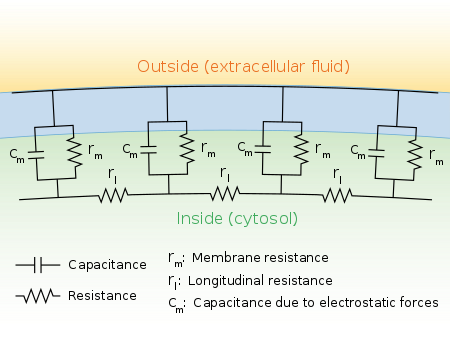
\includegraphics[scale=0.5]{Cable-Theory}
		\caption{A Teoria dos Cabos, para as ligações dos neurônios. Axônios e dentritos modelados como cabos elétricos - resistores e capacitores em sequência.}
		\label{Figura-1}
	\end{figure}
	
	\paragraph{}
	A teoria dos cabos modela o Axônio como um cabo, e, nas regiões machucadas do traumatismo, há o inchaço do axônio, como pode ser visto abaixo.
	\begin{figure}[h]
		\centering
		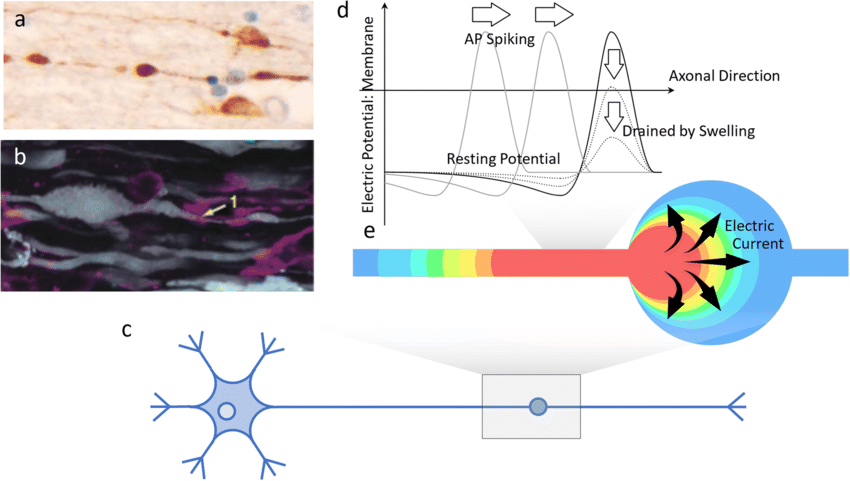
\includegraphics[scale=0.4]{Axonal-Swelling}
		\caption{Inchaço do Axônio devido ao traumatismo. Em \textbf{a} temos inchaços nas manchas vermelhas redondas. Em \textbf{b}, vemos inchaços mais longos, em grandes extensões. Os outros diagramas mostram o impacto do inchaço na condução da corrente elétrica no neurônio, acompanhando o axônio, e interferindo a condução na região do inchaço.}
	\end{figure}
	
	\paragraph{}
	
	A teoria dos cabos tem como principal modelo a equação diferencial dos cabos:
	\begin{equation}
		\frac{1}{r_{l}} \frac{\partial^{2} V}{\partial x^{2}} = c_{m} \frac{\partial V}{\partial t} + \frac{V}{r_m}
	\end{equation}
	
	Onde:
	\begin{itemize}
		\item $r_{l}$: A resistência intracelular do axônio ao longo de seu comprimento.
		\item $V$: Diferença de potencial ao longo do axônio com o ambiente externo.
		\item $x$: O comprimento do axônio, ou a distância a partir da origem do axônio.
		\item $r_{m}$: É a resistência da membrana do axônio.
		\item $c_{m}$: É a capacitância da membrana do axônio, em um segmento dele.
		\item $t$: Tempo, para a propagação dos pulsos neuronais.
	\end{itemize}
	
	\paragraph{}
	Que é aplicada ao inchaço com um modelo de um cabo contínuo com o aumento do raio do cabo em uma região. Esse aumento pode ser abrupto ou suave e, segundo o prof. Maia, a forma desse inchaço afeta a transmissão da informação neuronal de forma específica:
	
	\begin{itemize}
		\item Inchaços longos, que aumentam de diâmetro suavemente, não representam grande perda de transmissão de informação e são menos deletérios.
		\item Inchaços com aumento de diâmetro muito rápido, mesmo pequenos, representam perda de transmissão de informação e são muito deletérios.
		\item Inchaços com aumento de diâmetro rápido não apenas dificultam a transmissão de informação, como adicionam ruídos, reflexos e outros impactos nos sinais, que ainda ajudam a confundir a interação entre os neurônios.
	\end{itemize}
	
	\section{Conclusão: Fazendo Diagnósticos}
	O Modelo do Inchaço axonal, nos neurônios afetados pelo traumatismo craniano foi utilizado para mensurar o impacto de queda de transmissão de informações pelos neurônios nas regiões onde há traumatismo craniano. Ele pode ser estendido para fazer diagnósticos, entretanto, é necessário ter mecanismos de visualização do córtex, após o traumatismo, sem métodos invasivos e que exponham o cérebro dos pacientes de traumatismo.
\end{document}
